%%%%
\tetePremStssBiom

%%%% titre
\numeroActivite{3}

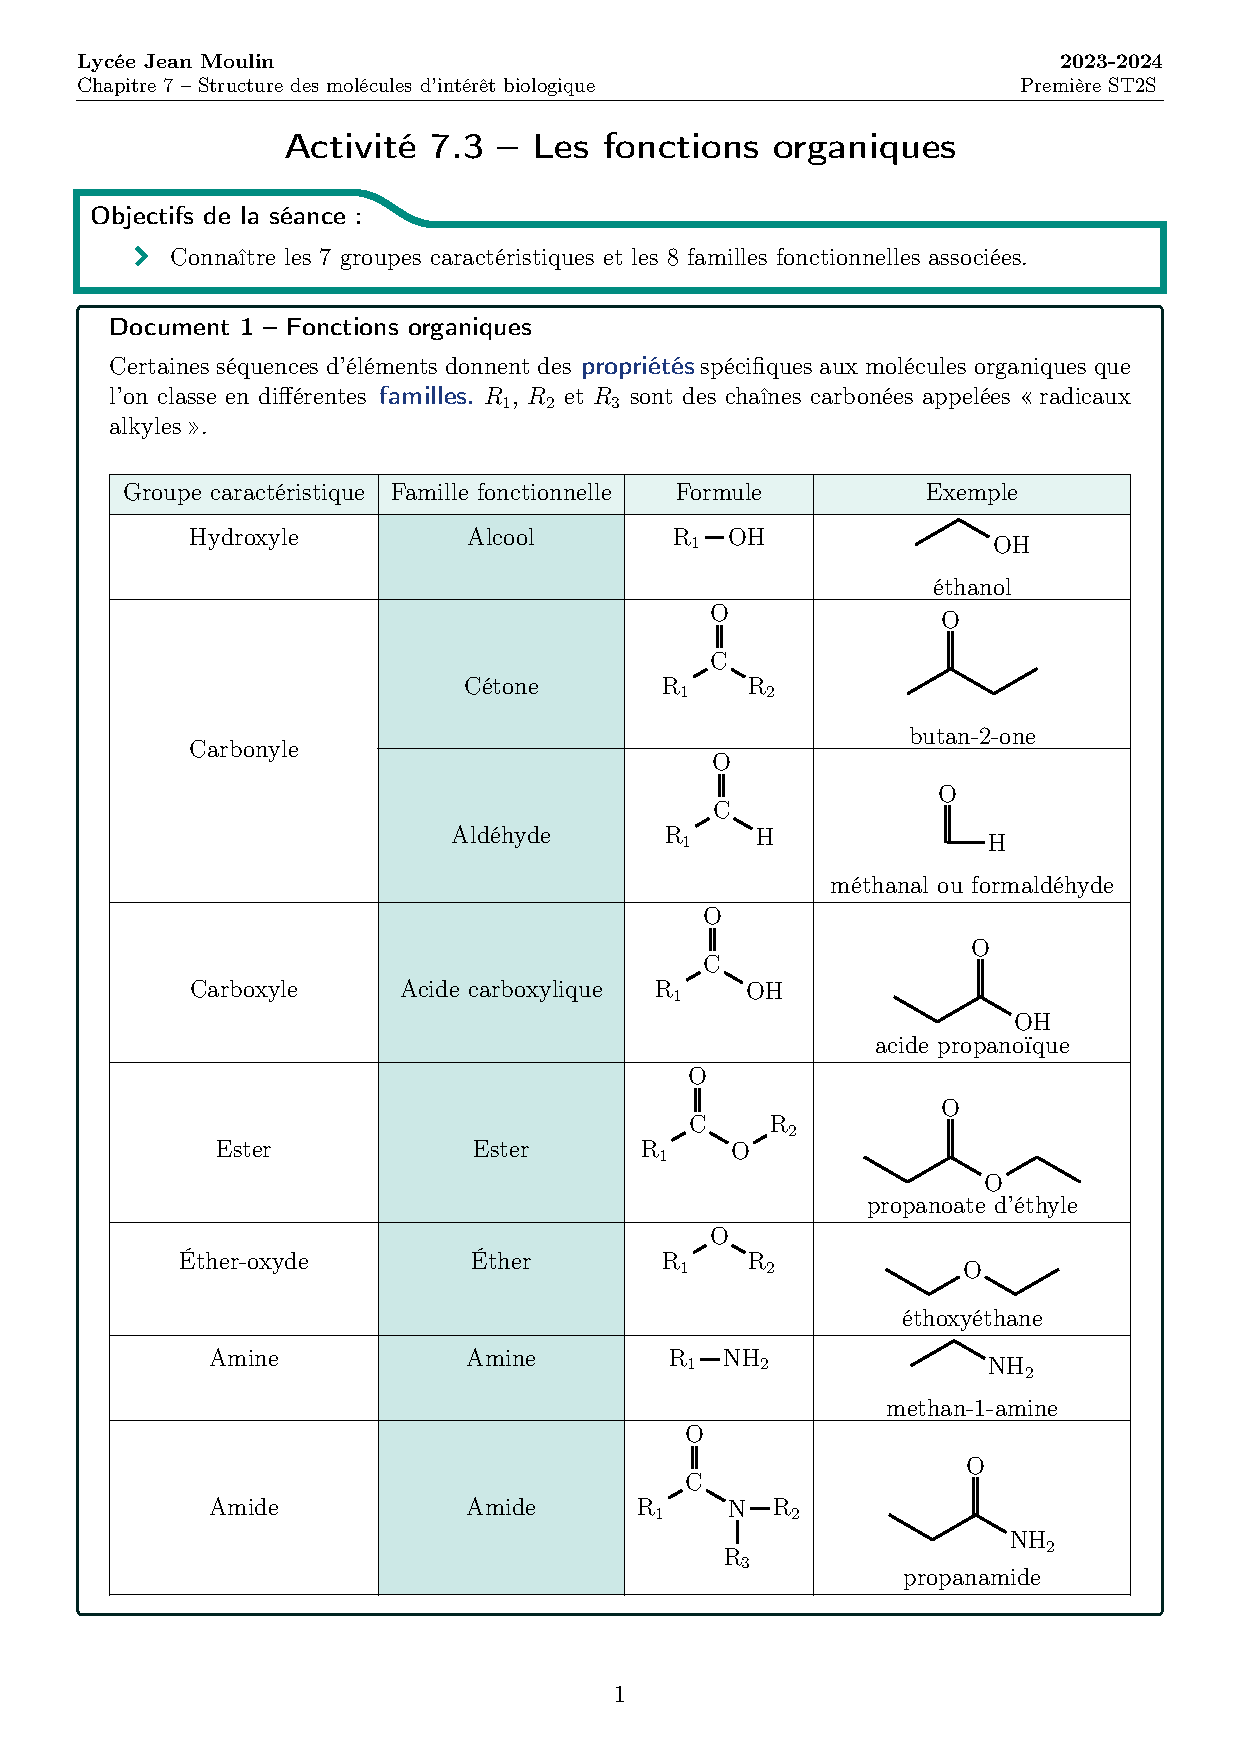
\includepdf{stssPremiere/C7_biomolecules/A7_fonction_orga_tableau}

\begin{doc}{Radicaux alkyle}{doc:A3_radicaux_alkyles}
  \begin{encart}
    Les \important{« radicaux alkyles »,} notés R, sont des morceaux de chaînes carbonées composées de liaisons simples avec des hydrogènes.
  \end{encart}

  \begin{tblr}{
    colspec = {|X[c] |X[c] |X[c] |X[c] |}, hlines,
    row{1} = {couleurPrim!20}
  }
    Méthyle & Éthyle & Propyle \\
    \vAligne{20pt} & & \\
  \end{tblr}
\end{doc}

\question{
  Identifier les fonctions organiques présentes dans les molécules suivantes
  
  \begin{center}
    \begin{tblr}{c c c c c}
      \chemfig{-[1] O -[-1] -[1]} &
      \chemfig{-[1] C (=[3] O) -[-1] OH} &
      \chemfig{-[1] !\ester -[1] -[-1] -[1]} &
      \chemfig{-[1] -[-1] -[1] (=[3] O) -[-1] H} &
      \chemfig{-[1] -[-1] -[1] (=[3] O) -[-1]} \\
      % 
      1 & 2 & 3 & 4 & 5
    \end{tblr}
  \end{center}
  \phantom{bla}
}{}{4}